 \documentclass[a4paper,12pt]{article}
\usepackage[a4paper,top=3cm,bottom=2cm,left=3cm,right=3cm,marginparwidth=1.75cm]{geometry}
\usepackage[brazil]{babel}
\usepackage[T1]{fontenc}
\usepackage[utf8]{inputenc}
\usepackage{amsmath}
\usepackage{MnSymbol}
\usepackage{wasysym}
\usepackage{hyperref}
\usepackage{color}
\definecolor{Blue}{rgb}{0,0,0.9}
\definecolor{Red}{rgb}{0.9,0,0}
\usepackage{esvect}
\usepackage{graphicx}
\usepackage{float}
\usepackage{indentfirst}
\usepackage{caption}
\usepackage{blkarray}
\newcommand\Mark[1]{\textsuperscript#1}
\usepackage{pgfplots}
\usepackage{amsfonts}
\usepackage[english, ruled, linesnumbered]{algorithm2e}
\usepackage{algorithmic}
\newtheorem{definicao}{Definição}[section]
\newtheorem{teorema}{Teorema}[section]

\title{Teoria de Grafos}
\author{Guilherme Philippi, Felipe Delfini Caetano Fidalgo}
\begin{document}
\maketitle
\tableofcontents

\section{Teoria de Grafos\label{sec:grafos}}
Esta seção tem como objetivo apresentar um breve resumo da \textit{teoria de grafos}, tema muito estudado por diversos matemáticos e aplicado em diversas áreas do conhecimento \cite{graphTheoryApplicationsBondy}.

\subsection{Descoberta (Eureka!)}
Costuma-se dizer que em 1736 é que a teoria teve início, com base no artigo publicado por Leonhard Euler sobre as 7 pontes de Königsberg \cite{euler:KOENIGSBERG} \cite{graphTheoryApplicationsBondy}, representada na Figura~\ref{fig:koni}. Segundo a história, os moradores daquela região perguntavam-se sobre a possibilidade de atravessar todas as sete pontes do local sem ter que repetir alguma delas. Esse é um problema muito usado para introduzir o tema \cite{problemsInMath} --- propõe-se o desafio de ligar todos os pontos de um desenho sem tirar o lápis do papel e sem passar duas vezes no mesmo ponto. Euler provou que isso não era possível ao formular matematicamente o problema, que deu origem a esta teoria.

\begin{figure}[H]
	\begin{center}
		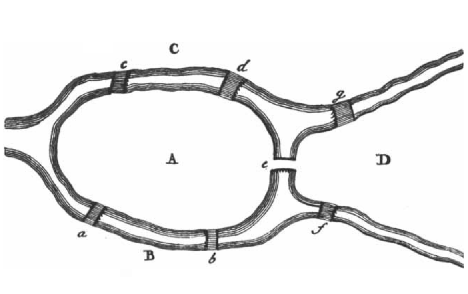
\includegraphics[width=0.7\linewidth]{figures/koenigsbern.png}
	\end{center}
	\caption{Ilustração original do problema \cite{euler:KOENIGSBERG}.}
	\label{fig:koni}
\end{figure}

A grande ideia de Euler foi abstrair o problema, vê-lo de uma forma elementar, como um conjunto de pontos conectados por curvas. Isso pode ser representado por um ``gráfico'', conforme a Figura~\ref{fig:koniGrafo} --- é daí a origem do termo em inglês "Graph", que é tradução literal de "Gráfico". Essa representação facilita a análise e a busca por uma solução. Com isso, Euler percebeu que só seria possível solucionar o problema se houvessem exatamente nenhum ou apenas dois pontos conectados por um número impar de curvas (ou pontes) \cite{euler:KOENIGSBERG}. Note que o caso de Koenigsberg, por tanto, não possui solução.

\begin{figure}[H]
	\begin{center}
		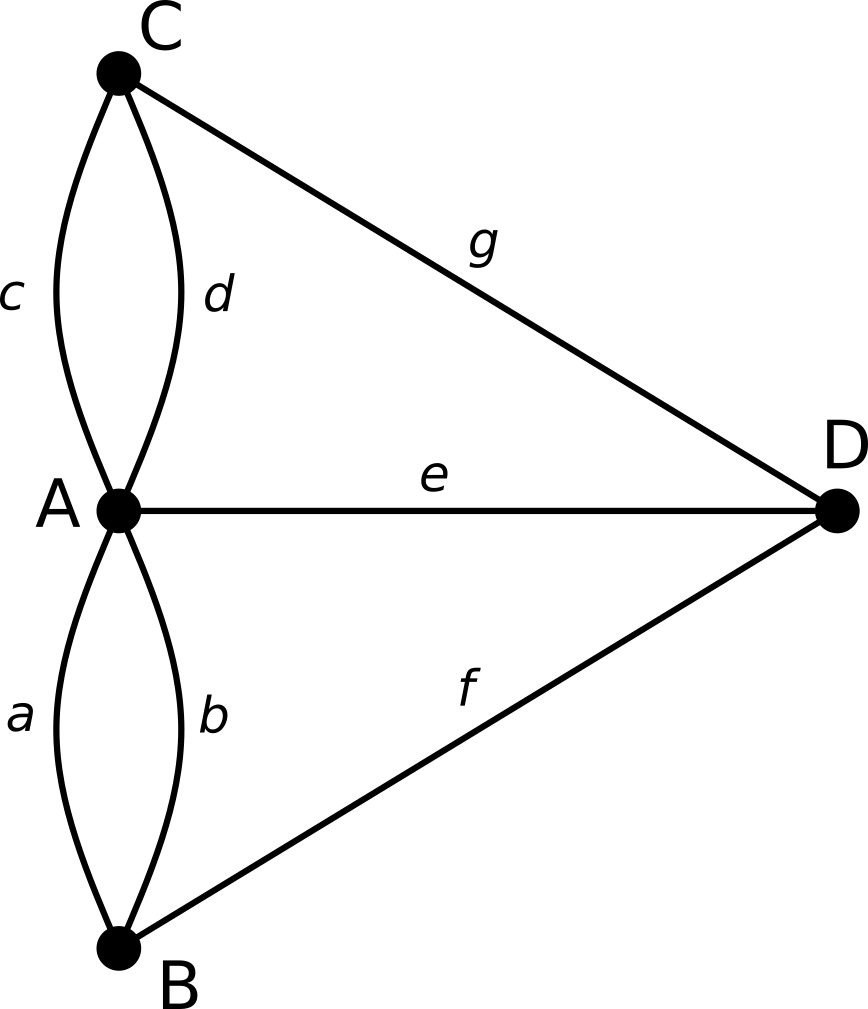
\includegraphics[width=0.32\linewidth]{figures/koenigsbernGrafo.png}
	\end{center}
	\caption{Representação em Grafos da ponte de Koenigsberg.}
	\label{fig:koniGrafo}
\end{figure}

Mas não podemos deixar todo o mérito com Euler. O conceito de grafo é muito intuitivo e foi proposto por diversas mentes brilhantes como formas de solucionar problemas que, em essência, são muito parecidos. Após Euler, a teoria foi redescoberta por Kirchhoff e Cayley \cite{graphTheoryFHarary}. Kirchhoff desenvolveu a teoria por volta de 1847, enquanto solucionava sistemas de equações lineares que relacionavam as correntes que passavam em cada malha fechada de um circuito elétrico \cite{kirchhoff1847ueber}, seguido por Cayley, em 1857, que estudava diferentes estruturas em bioquímica formadas por carbonos (sempre com quatro ligações químicas) e hidrogênios (com apenas uma ligação), onde conseguiu formular seu problema introduzindo o conceito de \textit{árvore} em grafos \cite{cayley1897theory}.  

Além dessas, muitas outras situações reais podem ser convenientemente representadas por simples diagramas contendo um conjunto de pontos e um conjunto de relações entre pares desses pontos. Por exemplo, podemos definir o conjunto $P = \{a,b,c\}$ das pessoas $a, b$ e $c$ e um conjunto $A = \{\{a,b\}, \{b,c\}\}$ como o conjunto de amizades entre essas pessoas --- no caso, $a$ é amigo de $b$, que é amigo de $c$, porém $a$ não é amigo de $c$. 
Este exemplo se torna muitíssimo útil quando se deseja estudar como a informação se propaga em redes sociais.

\begin{figure}[H]
	\begin{center}
		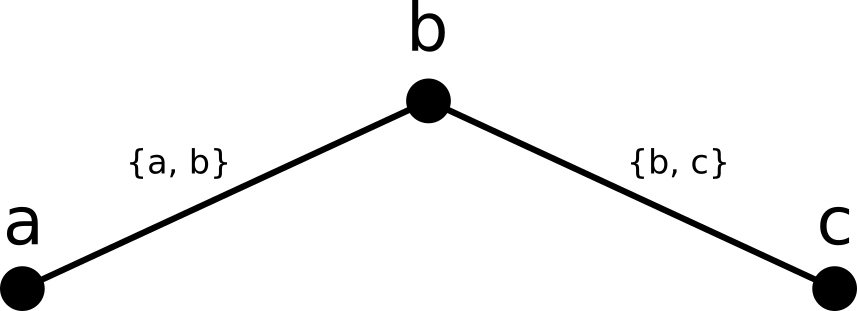
\includegraphics[width=0.35\linewidth]{figures/socialGraph.png}
	\end{center}
	\caption{Grafo representando o exemplo dado.}
	\label{fig:socialGraph}
\end{figure}

\subsection{Definição}

Não há um forte consenso sobre as terminologias usadas pelos autores sobre grafos \cite{graphTheoryFHarary}. Essa confusão é tanto gerada pela sua vasta disseminação em diversas áreas como pela enorme abstração que ela carrega. Cayley poderia chamar as relações entre pontos de ligações químicas enquanto Kirchhoff chamaria de curto-circuitos.
Faremos aqui um apanhado de definições sobre a teoria de grafos, mas não sobre toda ela. Essa é uma grande área da matemática e não nos cabe aborda-lá completamente. Trata-se apenas do essencial para que o leitor possa progredir sem ter que consultar uma bibliografia complementar sobre grafos.

Segue a definição geral.

\begin{center}
	\begin{minipage}{0.9 \linewidth}
		\textbf{Definição:} Um \textit{grafo} $G$ é uma tripla da forma $(V_G,E_G, \psi_{G})$, composta por um \textit{conjunto de vértices} $V_G$, um \textit{conjunto de arestas} $E_G$ e uma \textit{função de incidência} $\psi_{G}$ que, por sua vez, associa a cada elemento de $E_G$ um par não ordenado de elementos (nem sempre distintos) de $V_G$.
	\end{minipage}
\end{center} 

Nesse texto, porém, iremos abstrair a função de incidência $\psi_G$, pois entende-se que o conjunto de arestas $E_G$ é tal que, se $e \in E_G$, então $e = \{a, b\}$ onde $a, b \in V_G$. Fica implícita, por tanto, a associação dos elementos de  $E_G$ e $V_G$.
\\

A literatura utiliza termos distintos para os elementos de $V_G$ e $E_G$ \cite{graphTheoryFHarary}. Procuraremos nos referir a eles por \textit{vértices} e \textit{arestas}, respectivamente. Também, para um elemento $e \in E_G$, onde $e = \{u, v\}$, dizemos que $u$ e $v$ são \textit{vértices adjacentes}. Também dizemos que $u$ e $e$ são \textit{incidentes}, assim como $v$ e $e$. Se duas arestas distintas $e_1$ e $e_2$ são incidentes com um vértice em comum, dizemos que $e_1$ e $e_2$ são \textit{arestas adjacentes}. Seja um grafo com $m$ vértices e $n$ arestas, dizemos que este é um $(m, n)$ \textit{grafo}. Define-se o $(1,0)$ grafo como \textit{trivial}.

Utilizemos o recurso gráfico como ilustração: No $(3,2)$ grafo da Figura~\ref{fig:socialGraph}, os vértices $a$ e $b$ são adjacentes, assim como as arestas $\{a, b\}$ e $\{b, c\}$. Porém, os vértices $a$ e $c$ não são.

Existem muitas variações de grafos \cite{graphTheoryFHarary}. Perceba que a definição de grafo permite \textit{loops} (uma aresta da forma $e = \{v,v\}$, ou seja, $v$ é adjacente a si mesmo) e \textit{múltiplas arestas} (mais do que uma aresta ligando dois vértices). Grafos que permitem múltiplas arestas, mas não loops, são chamados de \textit{multigrafos}. Caso também permitam os loops, os chamamos de \textit{pseudografos}. Na Figura~\ref{fig:koniGrafo} (representando o problema das pontes de Koenigsberg) temos um multigrafo e a Figura~\ref{fig:pseudograph} ilustra um pseudografo.

\begin{figure}[H]
	\begin{center}
		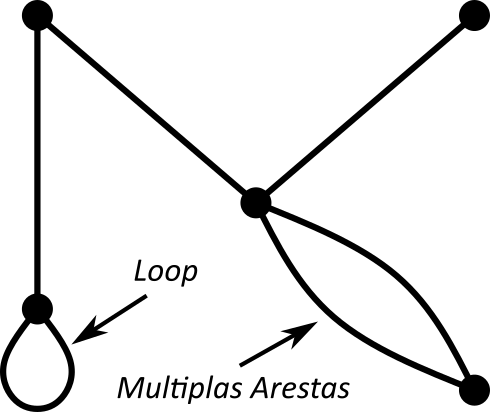
\includegraphics[width=0.28\linewidth]{figures/pseudograph.png}
	\end{center}
	\caption{Exemplo de pseudografo contendo 5 vértices e 6 arestas.}
	\label{fig:pseudograph}
\end{figure}

Nesse trabalho, não nos interessa o estudo de multigrafos ou pseudografos. Por isso adotaremos uma definição alternativa para grafos, visando restringir nossa aplicação, como segue:

\begin{center}
	\begin{minipage}{0.9 \linewidth}
		\textbf{Definição (2.0):} Um \textit{grafo} $G$ é uma dupla da forma $(V_G,E_G)$, composta por um conjunto não nulo e finito $V_G$ e outro conjunto finito $E_G$ de pares não ordenados de elementos \textbf{distintos} pertencentes a $V_G$.
	\end{minipage}
\end{center} 

\subsection{Outras Definições Importantes}

Dizemos que um grafo $G$ é \textit{rotulado} quando podemos distinguir seus $m$ vértices, nomeando eles, algo como $v_1, v_2, \dots, v_m$. Por exemplo, os grafos da Figura~\ref{fig:graphisomorphic} são rotulados, enquanto o grafo da Figura~\ref{fig:pseudograph} não é.

Dois grafos $G = (V_G, E_G)$ e $H = (V_H, E_H)$ são ditos isomorfos (escreve-se $G \cong H$) quando existe uma correspondência biunívoca entre os conjuntos de vértices $V_G$ e $V_H$ que preserve suas adjacências. A Figura~\ref{fig:graphisomorphic} ilustra essa situação, com a correspondência $v_i \longleftrightarrow v_i$.

\begin{figure}[H]
	\begin{center}
		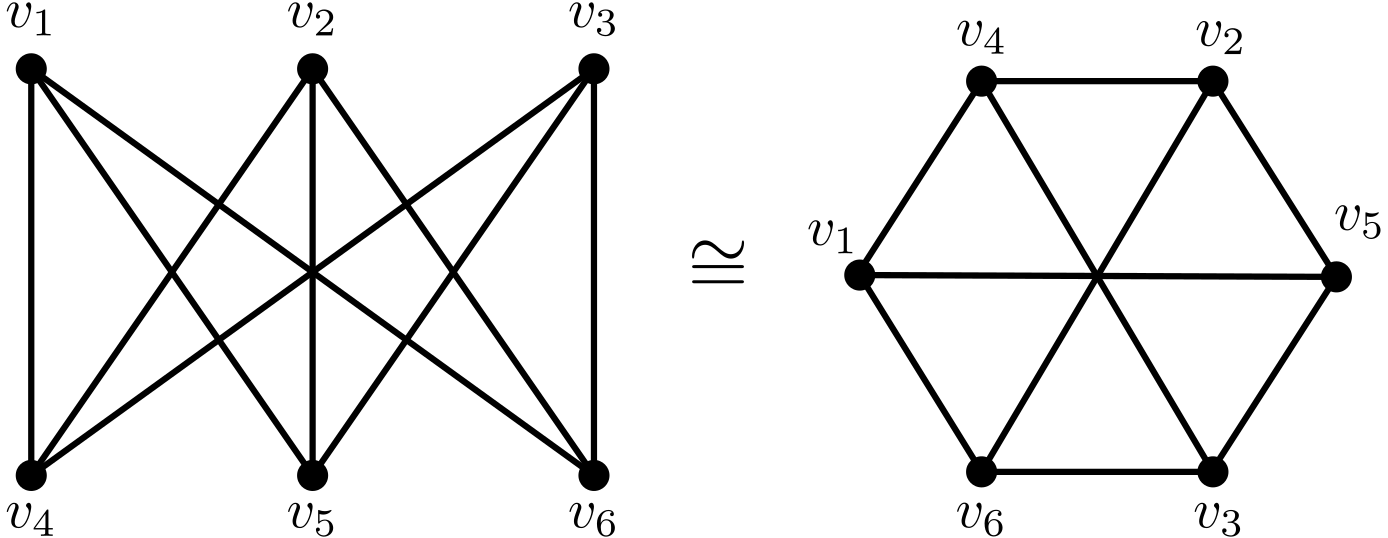
\includegraphics[width=0.6\linewidth]{figures/graphisomorphic.png}
	\end{center}
	\caption{Diferentes representações isomórficas de um (6, 9) grafo.}
	\label{fig:graphisomorphic}
\end{figure}

O isomorfismo é uma relação de equivalência em grafos. Fica claro que, por mais que seja útil, a representação gráfica de um grafo existe apenas como um apelo didático. A geometria formada pelos vértices é escolha de quem desenha. Vários são os casos em que problemas envolvendo grafos são facilmente solucionáveis apenas rearranjando a forma como se desenha. A resposta salta aos olhos.

\subsubsection*{Subgrafos}

Dizemos que o grafo $G_1 = (V_{G_1}, E_{G_1})$ é \textit{subgrafo} de $G = (V_G, E_G)$ se $V_{G_1} \subset V_G$ e $E_{G_1} \subset E_G$. Se $G_1$ é subgrafo de $G$, então $G$ é \textit{supergrafo} de $G_1$. Para qualquer $V \subset V_G$, existe um \textit{subgrafo induzido} $\langle V \rangle$ definido por $(V, E)$, onde $E \subset E_G$ contém todas as arestas $(v_1, v_2) \in E_G$ tal que $v_1, v_2 \in V$. 
Fica claro que dois vértices em $\langle V \rangle$ são adjacentes se, e somente se, forem também adjacentes em $G$.

Pode-se \textit{remover um vértice} $v$ de um grafo $G = (V_G, E_G)$, que resulta no subgrafo induzido $G - v = \langle V_G- v\rangle$. Da mesma forma, pode-se \textit{remover uma aresta} $e$ de um grafo $G = (V_G, E_G)$, resultando no grafo $G-e = (V_G, E_G - e)$.

\subsubsection*{Caminhos}

 
\begin{center}
	\begin{minipage}{0.9 \linewidth}
		\textbf{Laço:} Uma aresta $\{e_i, e_j\} \in E$ tal que $i = j$.
	\end{minipage}
\end{center}

Também, caso existam duas arestas iguais ($\{e_i, e_j\}$ e 
$\{e_j, e_i\}$, por exemplo, lembrando que $E$ é um conjunto de pares não ordenados), com as mesmas extremidades, estas recebem o nome de \textbf{arestas paralelas}.

\begin{center}
	\begin{minipage}{0.9 \linewidth}
		\textbf{Grafo simples}: Um grafo que não possui laços ou arestas paralelas.
	\end{minipage}
\end{center}

\begin{center}
	\begin{minipage}{0.9 \linewidth}
		\textbf{Grafo Completo:} É um grafo simples em que todo vértice é conectado a todos os outros vértices.
	\end{minipage}
\end{center}

\begin{figure}[H]
	\begin{center}
		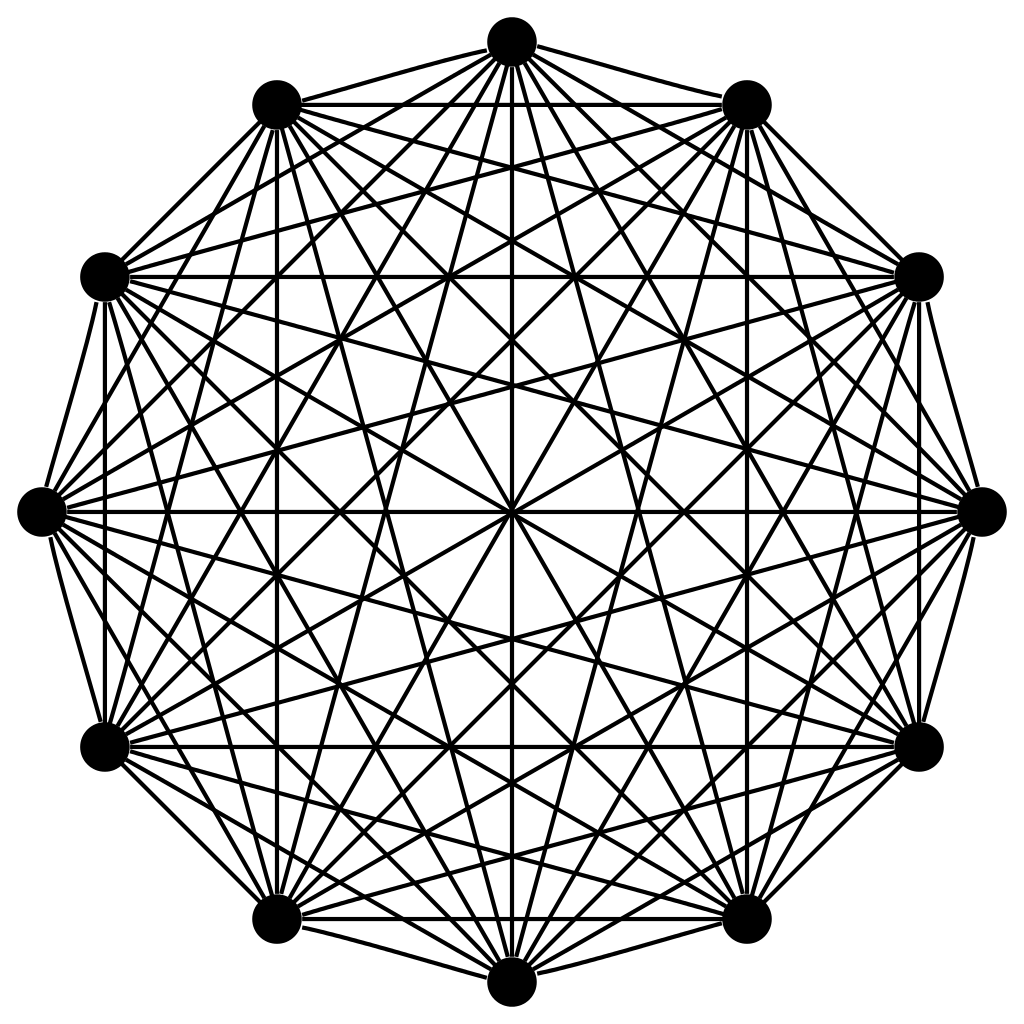
\includegraphics[width=0.4\linewidth]{figures/grafocompleto.png}
	\end{center}
	\caption{Diagrama de um grafo completo com 12 vértices ($|V| = 12$).}
	\label{fig:grafocompleto}
\end{figure}

Outro conceito que nos será de grande utilidade é o de subgrafo.
\begin{center}
	\begin{minipage}{0.9 \linewidth}
		\textbf{Subgrafo:} É um grafo resultante de um subconjunto de vértices e outro subconjunto de arestas de outro grafo. Isto é, seja $G = (V, E), G^\prime = (V^\prime, E^\prime)$ é dito um subgrafo de $G$ se $(V^\prime, E^\prime)$ é um grafo tal que $V^\prime \subseteq V$ e $E^\prime \subseteq E$.
	\end{minipage}
\end{center}

E, finalmente
\begin{center}
	\begin{minipage}{0.9 \linewidth}
		\textbf{$k$-Clique}: é um subgrafo $G^\prime$ com $k$ vértices tal que $G^\prime$ é completo.
	\end{minipage}
\end{center}

Em especial, também podemos interpretar as arestas como \textit{caminhos} e, se o fizermos, podemos pensar em alguma forma de métrica para esses caminhos. Esse pensamento da origem à nossa última definição de grafos, ditos \textit{ponderados}.

\begin{center}
	\begin{minipage}{0.9 \linewidth}
		\textbf{Grafo Ponderado:} É um grafo que possui uma função $d(E) \rightarrow \mathbb{R}$ associada, isto é, o grafo que possui valores numéricos atribuídos as suas arestas.
	\end{minipage}
\end{center}

\phantomsection
\addcontentsline{toc}{section}{Referências}

\bibliographystyle{unsrt}
\bibliography{references}

\end{document}
